\section{Systemmodelle}
\begin{figure}[htbp]
{\centering 
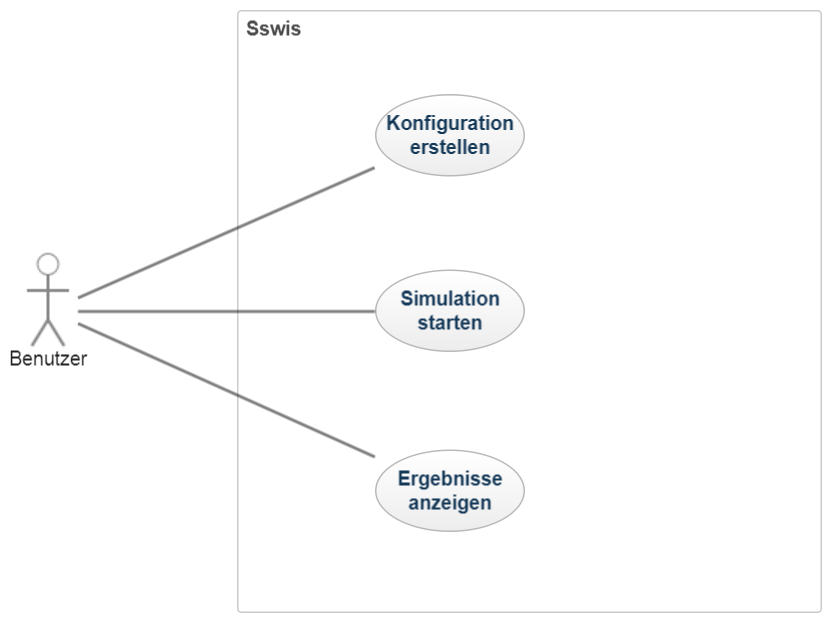
\includegraphics[width=0.9\textwidth]{Anwendungsfalldiagramme/usecase_sswis.png}
\caption{Das Programm in der Standardausführung} }
\bigskip
Sswis ist ein Simulator und gliedert sich als solcher in drei übergeordnete Anwendungen. Die Konfiguration der Rahmenbedingungen, das Starten der eigentlichen Simulation und das Abrufen der Ergebnisse. Die Interaktion mit dem Benutzer beschränkt sich im Wesentlichen auf die Konfiguration und die Anzeige der Ergebnisse. Die Simulation wird vom Benutzer initiiert und läuft anschließend ohne weiteres Einwirken von außen ab.

\end{figure}
\begin{figure}[htbp]
{\centering
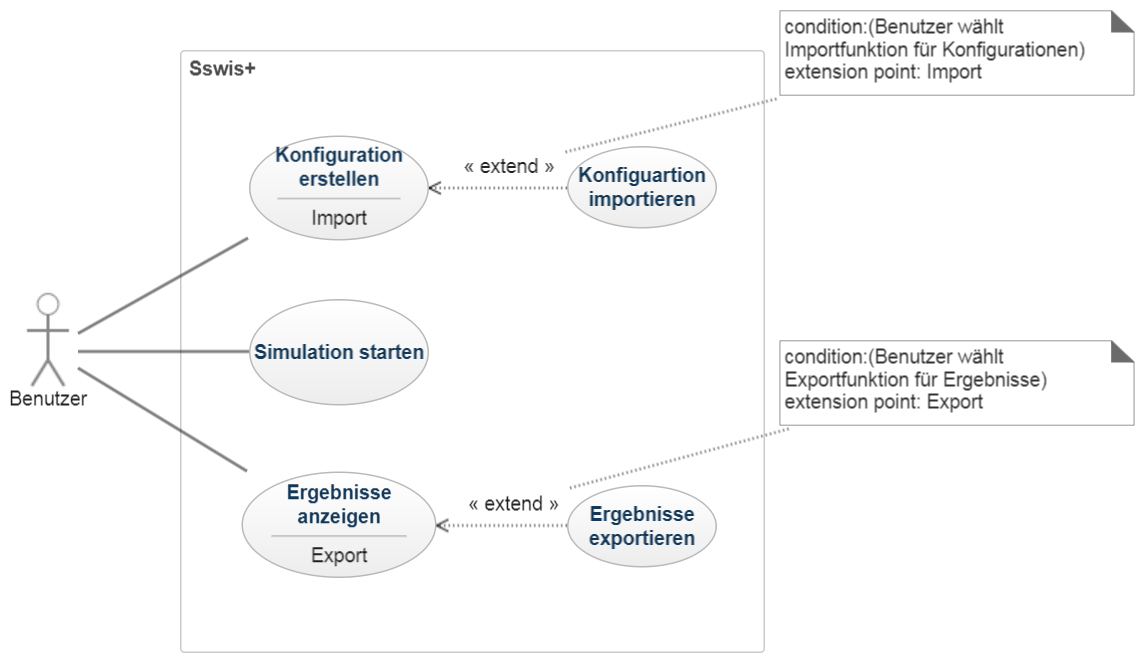
\includegraphics[width=1.1\textwidth]{Anwendungsfalldiagramme/usecase_sswis+.png}
\caption{Das Programm mit allen optionalen Funktionen} }
\bigskip

Zusätzlich zum Funktionsumfang von Sswis, erlaubt Sswis+ das Importieren von Konfigurationen und das Exportieren von Ergebnissen in Form jeweils einer Textdatei (z.B. CSV; Comma-separated values). Eine Datei zum Import einer Konfiguration wurde zu einem früheren Zeitpunkt durch den Konfigurationsassistenten erstellt (s.u.).

\end{figure}
\begin{figure}[htbp]
{\centering
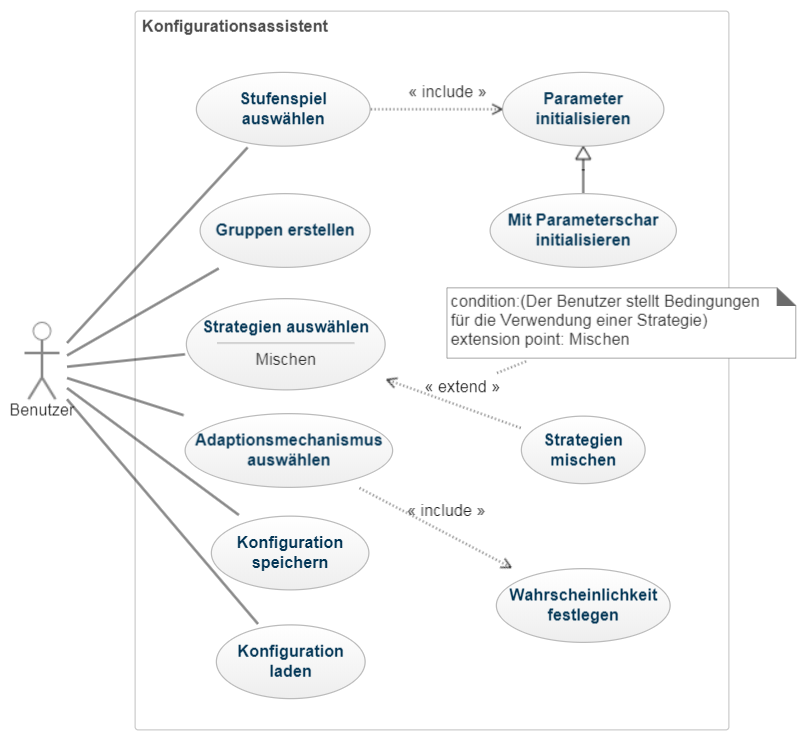
\includegraphics[width=1.0\textwidth]{Anwendungsfalldiagramme/usecase_config.png}
\caption{Der Konfigurationsassistent des Programms} }
\bigskip

\end{figure}